% ======================================================
% SLIDE CỦA BẠN BẮT ĐẦU TỪ ĐÂY
% (Nội dung không thay đổi)
% ======================================================

\begin{frame}
    \frametitle{Thách thức}
    \centering
    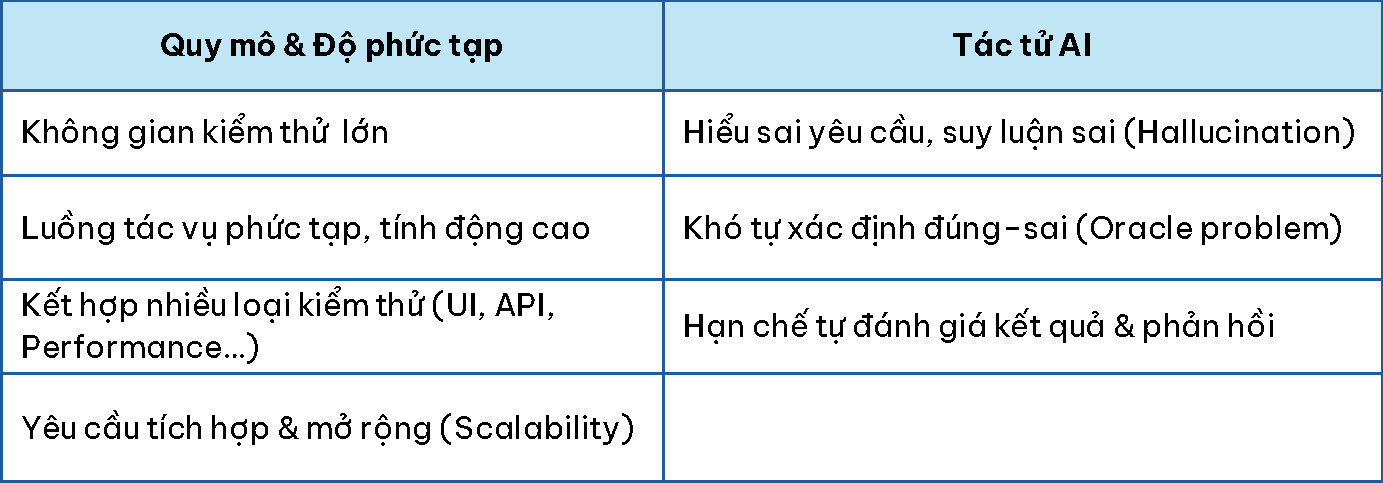
\includegraphics[width=\linewidth,height=0.8\textheight,keepaspectratio]{images/thachthuc}
    \vspace{0.8em}
    \small \textbf{Bảng 1:} Các thách thức  trong kiểm thử tự động sử dụng LLM hiện nay.
\end{frame}
% ======================================================
% KẾT THÚC SLIDE CỦA BẠN
% ======================================================


% ======================================================
% SLIDE: MỤC TIÊU NGHIÊN CỨU
% ======================================================
\begin{frame}
    \frametitle{Mục tiêu nghiên cứu}

    \begin{BulletTight}
        \item \textbf{Xây dựng hệ đa tác tử tích hợp LLM cho kiểm thử tự động}
        \begin{itemize}
            \item Khám phá tốt hơn trên không gian trạng thái lớn
            \item Phối hợp tác vụ hiệu quả, tránh trùng lặp
            \item Chuyên môn hoá tác tử → đầu vào chính xác, phát hiện lỗi sâu
            \item Linh hoạt thay đổi LLM theo vai trò
            \item Giảm lỗi suy luận nhờ SOP \& kiểm tra chéo
        \end{itemize}

        \vspace{0.4em}
        \item \textbf{Thiết kế cơ chế HITL tối ưu}
        \begin{itemize}
            \item Hỗ trợ bài toán oracle khó
            \item Giám sát \& điều chỉnh hành vi tác tử
            \item Tăng tốc \& tăng tỷ lệ phát hiện lỗi
            \item Học từ phản hồi người dùng hiệu quả (ít nhãn)
            \item Duy trì phản hồi xuyên suốt vòng đời kiểm thử
            \item Tối ưu chi phí ↔ hiệu quả
        \end{itemize}
    \end{BulletTight}
\end{frame}

